\documentclass[11pt]{article}
\usepackage[T1]{fontenc}
\usepackage[utf8]{inputenc}
\usepackage{amsmath,amsthm}
\usepackage{newtxtext,newtxmath}
\usepackage[margin=1.15in]{geometry}
\usepackage{microtype}
\usepackage{xcolor}
\usepackage{booktabs}
\usepackage{graphicx}
\graphicspath{{../}}
\renewcommand{\topfraction}{0.9}
\renewcommand{\floatpagefraction}{0.8}
\renewcommand{\textfraction}{0.1}
\usepackage[colorlinks=true,linkcolor=blue!50!black,citecolor=blue!50!black]{hyperref}

\newtheorem{theorem}{Theorem}
\newtheorem{conjecture}[theorem]{Conjecture}
\theoremstyle{definition}
\newtheorem{definition}[theorem]{Definition}
\theoremstyle{remark}
\newtheorem{remark}[theorem]{Remark}

\newcommand{\ds}{\mathsf{s}}

\title{Digit-Sum Reachability on the Lattice:\\
An Experimental Expedition from Brute Force to a Two-Line Criterion}
\author{Adam Benzan\thanks{Joint exploration with Claude (Anthropic). Scripts,
exact datasets, and the companion proof paper live in the project repository.}}
\date{July 2026}

\begin{document}
\maketitle

\begin{abstract}
Starting from $(0,0)$, a walker moves on $\mathbb{Z}^2$ through cells satisfying
$\ds(|x|)+\ds(|y|)\le N$, where $\ds$ is the digit sum (base $10$ unless noted).
We chronicle an experimental program on the reachable set: exact counts and the
fractal geometry of the region; a Cantor-like staircase in $N$ with cliffs at
multiples of $9$; an exact closed form in base $2$,
$Q(N)=\binom{2N+3}{N}$; a carry-free self-similar (``gastank'') decomposition
giving a polynomial-time exact solver; the asymptotic law
$\mathrm{reachable}/\mathrm{allowed\ in\ box}\sim c/\sqrt{N}$ with $c=3.84717(5)$
(refuting a tempting $\sqrt{15}$); and finally an exact two-line reachability
criterion, proved in a companion paper~\cite{criterion}, which subsumes every structure met along
the way and reduces all counting to a one-dimensional walk recursion. We keep the
narrative in expedition order, including two instructive false summits.
\end{abstract}

\section{The problem}

A cell $(x,y)\in\mathbb{Z}^2$ is \emph{allowed} iff $\ds(|x|)+\ds(|y|)\le N$;
the \emph{reachable set} is the $4$-connected component of the origin within the
allowed set. Write $f(N)$ for its size and $Q(N)$ for the size of its closed-quadrant
part. The canonical instance is $N=19$:
\[
f(19)=102{,}485,\qquad \text{bounding box } [-298,298]^2 ,
\]
the box ending exactly at the first \emph{axis cliff}: $\ds(299)=20$ makes the
entire column $|x|=299$ forbidden. The region is $4$-fold symmetric, diamond-like at
large scale, pierced by rectangular ``death zones'' and nested self-similar
triangular voids (Figure~\ref{fig:reach}).

\begin{figure}[htbp]
\centering
\includegraphics[width=0.55\textwidth]{digitsum_reach.png}
\caption{The reachable set at $N=19$ ($102{,}485$ cells, box $[-298,298]^2$):
diamond envelope, rectangular death zones, and the nested ``tri-force''
triangular voids from the self-similarity of digit sums at powers of ten.}
\label{fig:reach}
\end{figure}

\subsection*{Allowed versus reachable}
Each row $y$ of the allowed set is the one-dimensional set
$\{x:\ds(|x|)\le N-\ds(|y|)\}$, so the allowed set factors through a family of
$1$-D threshold sets. Counting allowed cells in the bounding box at $N=19$ gives
$166{,}973$, versus $102{,}485$ reachable: a gap of $64{,}488$ cells
($38.6\%$) that satisfy the constraint but are cut off behind carry cliffs ---
\emph{islands}. The canonical island: $(300,0)$ is allowed ($\ds=3$) but hidden
behind the forbidden column $x=299$. Figure~\ref{fig:signal} shows the 1-D
digit-sum signal whose threshold crossings generate the cliffs.

\begin{figure}[htbp]
\centering
\includegraphics[width=\textwidth]{digitsum_signal.png}
\caption{The digit-sum signal $\ds(x)$ for $x=0..300$ against the threshold
$N=19$ (red). Reachability along the axis ends at the first crossing,
$\ds(299)=20$; each row of the 2-D problem sees this same signal at a reduced
threshold.}
\label{fig:signal}
\end{figure}

\section{The staircase in \texorpdfstring{$N$}{N}}\label{sec:staircase}

Exact counts as $N$ grows show a descending, Cantor-like pattern in the ratio
$f(N)/\text{allowed-in-box}$, with cliffs exactly at $N\in\{9,18,27,36\}$ --- the
thresholds at which the box first jumps a decade.

\begin{center}
\begin{tabular}{rrrrr}
\toprule
$N$ & $f(N)$ & allowed (box) & ratio & box \\
\midrule
 8 & 145 & 145 & 1.0000 & $\pm 8$ \\
 9 & 505 & 649 & 0.7781 & $\pm 18$ \\
17 & 14{,}785 & 18{,}265 & 0.8095 & $\pm 98$ \\
18 & 47{,}905 & 73{,}885 & 0.6484 & $\pm 198$ \\
19 & 102{,}485 & 166{,}973 & 0.6138 & $\pm 298$ \\
26 & 1{,}309{,}537 & 1{,}885{,}501 & 0.6945 & $\pm 998$ \\
27 & 4{,}216{,}357 & 7{,}552{,}009 & 0.5583 & $\pm 1998$ \\
35 & 117{,}109{,}345 & 190{,}327{,}945 & 0.6153 & $\pm 9998$ \\
36 & 377{,}329{,}873 & 761{,}526{,}445 & 0.4955 & $\pm 19998$ \\
\bottomrule
\end{tabular}
\end{center}

Within each decade the topology is fixed and holes fill in monotonically; each new
decade adds an outer, rescaled copy of the previous decade's pattern
(Figures~\ref{fig:ratio} and \ref{fig:peaktrough}). The ratio
minimum falls two steps \emph{after} each cliff ($N=11,20,29$), not at it.

\begin{figure}[htbp]
\centering
\includegraphics[width=\textwidth]{digitsum_ratio_extended.png}
\caption{The Cantor-like staircase: reachable count, allowed-in-box count, and
their ratio for $N\le 28$, with cliffs at $N=9,18,27$ where the bounding box
jumps a decade.}
\label{fig:ratio}
\end{figure}

\begin{figure}[htbp]
\centering
\includegraphics[width=\textwidth]{digitsum_peak_trough.png}
\caption{First-of-decade (trough) versus last-of-decade (peak) shapes for
decades 2 and 3. The $N=11$ trough is the $N=20$ trough rescaled; the recursion
made visible.}
\label{fig:peaktrough}
\end{figure}

\section{The monotone lemma}\label{sec:monotone}

A BFS-depth experiment found \emph{detour} $:=$ geodesic $-\;(|x|+|y|)$ to vanish
on every reachable cell: whatever is reachable at all is reachable by a monotone
staircase. Equivalently, in the quadrant,
\[
R(x,y)=\text{allowed}(x,y)\wedge\bigl(R(x{-}1,y)\vee R(x,y{-}1)\bigr)
\]
reproduces full undirected reachability. Verified for $N\le 22$ (base 10) and for
bases $2\text{--}5$; later \emph{proved} as a corollary of the criterion of
\S\ref{sec:criterion}. Connectivity failures are always total (islands), never
partial (no cell requires a detour); see Figure~\ref{fig:depth}. Practically, the
lemma converts BFS into a vectorized row sweep, ${\sim}100\times$ faster --- the
workhorse for everything below.

\begin{figure}[htbp]
\centering
\includegraphics[width=0.48\textwidth]{digitsum_depth.png}\hfill
\includegraphics[width=0.48\textwidth]{digitsum_detour.png}
\caption{Left: cells colored by geodesic (BFS) distance from the origin at
$N=19$. Right: detour $=$ geodesic $-\,(|x|+|y|)$, identically zero --- the
observation that became the monotone lemma and, eventually, the criterion.}
\label{fig:depth}
\end{figure}

\section{Base 2: an exact closed form}\label{sec:base2}

In base $2$ the quadrant count is a single binomial coefficient:
\[
Q_2(N)=\binom{2N+3}{N},\qquad
f_2(N)=4\binom{2N+3}{N}-2^{N+3}+5 ,
\]
first verified for $N\le 15$ (the $N=15$ value \emph{predicted before} a
$4.3\times10^9$-cell sweep confirmed it), later \emph{proved} from the
criterion: interleaving the bits makes reachability a $\pm1$-path condition
whose even-checkpoint constraint collapses, by parity, to the uniform barrier
``never reach $+2$'', and reflection at level $2$ telescopes the count to
$\binom{2k}{k-1}+\binom{2k}{k-2}$ --- the allowed cells of the top two weight
layers, with an explicit \emph{surfacing map} bijection (complement prefixes up
to first hits of level $-2$). The allowed-set side is classical,
$\tfrac12\bigl(4^{N+1}-\binom{2N+2}{N+1}\bigr)$, so the island count is closed-form by
subtraction, and
\[
\frac{Q_2(N)}{\text{allowed}}\;\longrightarrow\;\frac{4}{\sqrt{\pi N}} .
\]
The ratio tends to \emph{zero}: there is no finite asymptotic density. $Q_2$ is
OEIS A002054 (ballot numbers), pointing to a lattice-path bijection; the base-10
sequence $f(N)$ was not then in OEIS. Figure~\ref{fig:strip} compares the region across
bases: base 2 is densest and nearest a solid diamond (carries at every step weave
fine cliffs), while larger bases have rarer but more violent carries, punching
larger holes.

\begin{figure}[htbp]
\centering
\includegraphics[width=\textwidth]{digitsum_strip.png}
\caption{Reachable regions in bases $2,3,4,5,10$, with $N$ chosen so each has
axis reach ${\sim}\pm250$--$500$. Base 10 is the noisiest member of the family.}
\label{fig:strip}
\end{figure}

\section{Gastanks: the carry-free decomposition}\label{sec:tanks}

\begin{definition}[Tank, wall, weir, wetting front]
A \emph{tank} $T_k(K)$ is a block $[0,10^k)^2$ in local coordinates with budget
$K$: local cell $(u,v)$ allowed iff $\ds(u)+\ds(v)\le K$. Since digit sums are
carry-free inside a block, the child at digit position $(i,j)$ is exactly
$T_{k-1}(K-i-j)$: budgets step down by one per digit, with no corrections, ever.
A \emph{wall} is the trailing-nines seam between sibling tanks (digit-sum cost
$9s$ at sibling scale $s$); carries \emph{are} walls. A \emph{weir} is the
passable part of a wall, $\{v:\ds(v)\le K_{\mathrm{left}}-9s\}$ --- itself a 1-D
threshold set one scale down. A \emph{wetting front} is the set of edge cells
through which flow passes; fronts are Cantor-dust-like with up to ${\sim}9^{k-1}$
intervals.
\end{definition}

Equivalently, in \emph{terrain} coordinates (elevation $=\ds(x)+\ds(y)$,
waterline $=N$): walls are ridges, weirs are notches dipping below the waterline,
islands are submerged basins sealed off by ridges that never dip. All four terms
appear together in a single real strip of the $N{=}19$ plane in
Figure~\ref{fig:glossary}.

Flooding tanks recursively --- passing fronts over weirs, with fronts hash-consed
as interned $10$-tuples of child fronts (a DAG; never expanded) --- gives an exact
solver whose distinct-state count grows only polynomially (${\sim}N^{3.3}$).
Benchmarks (cold start, cross-checked outputs):

\begin{center}
\begin{tabular}{rrrrrl}
\toprule
$N$ & BFS (set) & BFS (grid) & monotone DP & tanks & $f(N)$ \\
\midrule
26 & 1.31 s & 1.19 s & 0.009 s & 0.002 s & $1.3\times10^{6}$ \\
28 & --- & 8.55 s & 0.053 s & 0.003 s & $9.0\times10^{6}$ \\
36 & --- & --- & 1.98 s & 0.008 s & $3.8\times10^{8}$ \\
90 & --- & --- & --- & 0.13 s & $2.5\times10^{20}$ \\
360 & --- & --- & --- & 16.2 s & ${\sim}10^{89}$ \\
630 & --- & --- & --- & 144 s & ${\sim}10^{140}$ \\
\bottomrule
\end{tabular}
\end{center}

The first three methods are all $O(\text{area})=O(10^{2N/9})$; the tank solver is
polynomial in $N$. Per residue $N\bmod 9$, the sequence $Q$ admits no C-finite
recurrence of order $\le 13$ and no polynomial-coefficient recurrence of order
$\le 6$, degree $\le 8$ (higher orders untested) --- but the \emph{allowed}
count fails identically, so base 10 lacks base 2's central-binomial collapse
rather than being intrinsically wilder.

\begin{figure}[htbp]
\centering
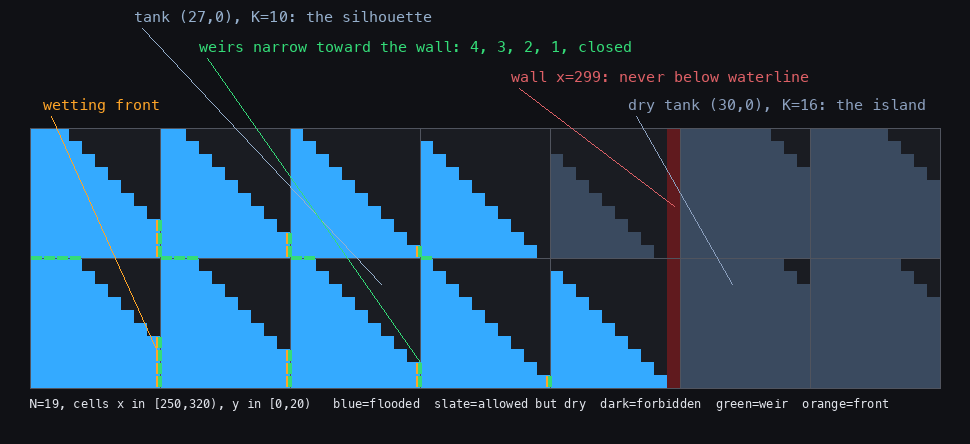
\includegraphics[width=\textwidth]{digitsum_glossary.png}
\caption{The glossary in one strip: cells $x\in[250,320)$, $y\in[0,20)$ at
$N=19$. Scale-1 tanks with budgets $K=19-\ds(a)-\ds(b)$ show their triangular
silhouettes (blue: flooded; slate: allowed but dry; dark: forbidden). Weirs
(green) narrow $4,3,2,1$ and then close as budgets shrink toward the wall at
$x=299$ (red), whose column never dips below the waterline --- so tank $(30,0)$,
despite its generous $K=16$, stays dry: the canonical island containing
$(300,0)$. Orange marks the wetting front on each tank's exit edge.}
\label{fig:glossary}
\end{figure}

\section{The constant \texorpdfstring{$c$}{c}: two false summits}\label{sec:c}

On the \emph{peak line} $N\equiv 8 \pmod 9$, set
$c_N=\sqrt{N}\cdot\mathrm{reachable}/\mathrm{allowed\ in\ box}$ (the box is
the $k$-digit square; on the peak line it exceeds the reachable bounding box
only by the forbidden row and column at coordinate $10^k-1$, digit sum $N+1$,
so the allowed counts coincide; the unrestricted allowed set is infinite, so
the qualification is required).

\emph{False summit 1: $\sqrt{15}$.} Pair extrapolations through $N=629$ landed
within $1.3\times10^{-5}$ of $\sqrt{15}=3.87298$. But exact data to $N=989$
(tank solver, $15$M states) showed $c_N$ \emph{cresting} at $3.86931$ near
$N\approx650$ and then descending with accelerating increments ---
$\sqrt{15}$ exceeds every value ever attained. The agreement was a crossing
artifact of two competing correction terms.

\emph{False summit 2: $c=3.865\pm0.004$.} With data ending at $N=989$, model
fits (calibrated on base 2, where naive $1/N$-polynomial extrapolation misses
$4/\sqrt{\pi}$ by $2\times10^{-2}$) gave $3.865(4)$. The criterion of
\S\ref{sec:criterion} later allowed evaluation at $k=16{,}000$
($N=143{,}999$): the descent continues far past the old horizon, and
\[
c \;=\; 3.84717(5)
\]
--- precisely where earlier ``degenerate'' power-law fits had pointed. The crest
and both apparent correction families --- what was \emph{then} read as a
geometric-per-decade term with ratio ${\sim}0.91$ (an interpretation later
withdrawn in \S\ref{sec:rho}) and a slow power tail --- are finite-$k$
features of one exact model.
Bases $3,4,5$ show the same crest-then-descend shape; base 2
($c_2=4/\sqrt{\pi}$, approach from above) is the degenerate case.

\emph{The summit itself.} The criterion converts the peak-line count into a
stay-nonnegative probability of the reflected tent walk, and the Sparre
Andersen identity (Wiener--Hopf factorization in combinatorial form) then gives
the constant in closed form:
\[
c_b=\frac{2\sqrt{b-1}}{\sqrt{\pi}}
\exp\!\Bigl(\tfrac12\sum_{n\ge1}\frac{p_n}{n}\Bigr)
=\frac{2\sqrt{b-1}}{\sqrt{\pi}}
\exp\!\Bigl(-\frac{1}{4\pi}\int_{-\pi}^{\pi}
\log\bigl(1-\varphi_b(\theta)\bigr)\,d\theta\Bigr),
\]
with $p_n=\Pr(S_n{=}0)$ and
$\varphi_b(\theta)=\bigl(\sin(b\theta/2)/(b\sin(\theta/2))\bigr)^2$. Base 2
collapses by hand ($\sum p_n/n=2\log2$, $c_2=4/\sqrt{\pi}$ exactly); series and
integral evaluations agree to nine decimals in every base; and
$c_{10}=3.847174895\ldots$ matches the walk-DP value. The identity was verified
coefficientwise against a barrier DP to $10^{-15}$.

\section{The spectral expedition}\label{sec:spectral}

Instrumenting the flood recursion and normalizing tank states as
$(\text{depth},\, d,\ \text{front classes})$ with $d=9k-K$ (offset of the
waterline from the tank's mean elevation) yields, empirically:

\begin{enumerate}
\item \textbf{Exact fixed point.} The shallow census is \emph{identical} ---
integer-for-integer --- across all peak-line $N$ tested ($116$--$404$), at every
instrumented depth. All $N$-dependence lives in the deepening diffusive interior.
\item \textbf{Closure.} Transition profiles are well-defined functions of
truncated front signatures ($577/651$ classes unambiguous; failures only at
deeply submerged $d\le-35$); classes per offset saturate at $24$. The active band
is one-sided: no active tank has $d>1$.
\item \textbf{Spectrum.} The truncated transfer matrix gives $\lambda_1\to95.2$
(toward the trivial $100$) and $\lambda_2/\lambda_1$ rising
$0.58\to0.78\to0.86$ with truncation depth. \emph{(The interpretation of this as
approaching the observed correction ratio ${\sim}0.91$ was later withdrawn: the
$0.91$ in $c_N$ is a power-family fitting artifact, not an eigenvalue --- see
\S\ref{sec:rho}. The matrix gap itself remains a genuine property of the
tank-count operator.)}
\end{enumerate}

The $d$-walk steps by $(i+j)-9$ per scale: a Markov-additive process whose
continuum spectrum is the power-law correction family of \S\ref{sec:c}.

\section{The reachability criterion}\label{sec:criterion}

A scalar Wiener--Hopf ``warm-up'' --- modelling reachability as the $d$-walk
surviving below the census barrier $d\le1$ --- reproduced base 2's constant to
$4\times10^{-5}$ with no fitted parameters. Testing whether the model is
\emph{literally} true:

\begin{theorem}[Reachability criterion; proof in \cite{criterion}]
In base $b$, threshold $N$, $k=\lfloor N/(b{-}1)\rfloor+1$: a quadrant cell
$(x,y)$ is reachable iff every proper digit-prefix pair
\emph{(lengths $1\le s<k$)} satisfies
\[
\ds\bigl(x\langle s\rangle\bigr)+\ds\bigl(y\langle s\rangle\bigr)\;\le\;
N-(b{-}1)(k{-}s)+1 ,
\]
and $\ds(x)+\ds(y)\le N$.
\end{theorem}

Zero mismatches against exhaustive reachability across bases $3,5,10$; integer
equality with the tank solver's $Q(N)$ up to $N=989$. The proof is elementary:
\emph{necessity} because any entry into a cell's scale-$m$ ancestor tank crosses
a trailing-nines wall, entries from the left/below certifying the
\emph{neighbor's} wall --- one digit cheaper via $\ds(X)\le\ds(X{-}1)+1$, whence
the $+1$ slack; \emph{sufficiency} by an explicit L-path to the ancestor tank's
corner --- worst cells $(a{-}1)\underline{9\cdots9}$ and
$a+(c{-}1)\underline{9\cdots9}$, allowed exactly under the criterion bound ---
followed by recursion inside the tank at threshold $N-a-c$. The two $+1$'s
coincide; the criterion is sharp. The monotone lemma follows as a corollary.

Consequences: counting reduces to a $1$-D walk recursion ($O(k^2b^2)$, i.e.\
$O(k^2)$ for fixed base ---
microseconds at any $N$); the constant $c$ is a one-boundary survival constant of
the centered tent walk, i.e.\ a kernel-method/Wiener--Hopf object with an
explicit (if unlovely) analytic characterization; and the $24$-class front
dynamics of \S\ref{sec:spectral}, while real as $2$-D geometry, is
count-irrelevant --- reachability depends only on ancestor budgets.

\section{The \texorpdfstring{$\rho\approx0.91$}{rho = 0.91} structure: a
masquerade}\label{sec:rho}

The criterion makes $c_k$ exactly computable, and its correction structure is a
power family
\[
c_k \;=\; c\,\Bigl(1+\frac{\alpha}{\sqrt{k}}+\frac{\beta}{k}
+\frac{\gamma}{k^{3/2}}+\cdots\Bigr),
\qquad \alpha=\frac{1}{\sigma\sqrt{2\pi}}=0.098213\ldots,
\]
where $\sigma^2=(b^2-1)/6$ is the variance of a tent step, with $\alpha$
forced by the denominator alone: the lattice atom $\Pr(S_k{=}0)$ in the
allowed-count normalization $(1-p_k)/2$ ($1/\sqrt{\pi}$ exactly in base~2).
The numerator contributes no $k^{-1/2}$ term: writing $w=1-z$ and
$G(z)=\tfrac12\sum_n p_nz^n/n$, the Sparre Andersen generating function of the
stay-nonnegative probabilities $q_k$ is $w^{-1/2}e^{G(z)}$, and since
$p_n\sim\alpha n^{-1/2}$ the leading singular part of $G$ is
$-\alpha\sqrt{\pi}\,w^{1/2}$, whose product with the prefactor is the analytic
constant $w^{-1/2}\cdot w^{1/2}=1$, contributing nothing to $[z^k]$.

Pushed one order further, the same expansion gives $\beta$ in closed form
(\texttt{digitsum\_beta.py}). Let $K=e^{G(1)}$, so that
$c_b=2\sqrt{b-1}\,K/\sqrt{\pi}$, and
$\rho_1=\sum_{n\ge1}\bigl(p_n-\alpha n^{-1/2}\bigr)$, convergent since
$p_n-\alpha n^{-1/2}=O(n^{-3/2})$. Expanding $\mathrm{Li}_{3/2}$ at $z=1$
gives $G(z)=\log K-\alpha\sqrt{\pi}\,w^{1/2}
-\tfrac12\bigl(\alpha\,\zeta(\tfrac12)+\rho_1\bigr)w+O(w^{3/2})$, and
singularity analysis of $w^{-1/2}e^{G}$ yields
$q_k=K(\pi k)^{-1/2}\bigl(1+u_1/k+O(k^{-2})\bigr)$ with
$u_1=-\tfrac18+\tfrac14\bigl(\alpha\,\zeta(\tfrac12)+\rho_1\bigr)
-\tfrac14\pi\alpha^2$. Reachability needs endpoint $\ge1$, so the endpoint
atom $r_k=\Pr(S_1,\dots,S_{k-1}\ge0,\;S_k=0)$ is subtracted; by the
Spitzer--Baxter identity its generating function is the $u^0$ coefficient of
$\exp\sum_n\frac{z^n}{n}\,\mathbb{E}[u^{S_n};S_n\ge0]$, namely $e^{2G(z)}$
(verified coefficientwise to $10^{-17}$; $C_{k+1}/4^k$ in base~2), so
$r_k\sim K^2\alpha\,k^{-3/2}$. Assembling
$c_k=2\sqrt{(b-1)k-1}\,(q_k-r_k)/(1-p_k)$ with
$K\alpha\sqrt{\pi}=K/(\sigma\sqrt2)$,
\[
\beta\;=\;\Bigl(1-\frac{\pi}{4}\Bigr)\alpha^2-\frac{K}{\sigma\sqrt2}
-\frac18-\frac{1}{2(b-1)}+\frac{\alpha\,\zeta(\frac12)+\rho_1}{4}.
\]
In base~2 everything is explicit ($K=2$, $G=\log\bigl(2/(1+\sqrt{w})\bigr)$,
so $\alpha\zeta(\frac12)+\rho_1=-1$): $\beta_2=1/\pi-25/8=-2.80669\ldots$.
In base~10 the formula gives $\beta=-0.414716$, and the power family fitted
to the exact $c_k$ on $k\in[300,1500]$ with $\alpha$ pinned returns
$-0.414716$; with $\alpha$ and $\beta$ both pinned, two fitted higher terms
reproduce $c_k$ to rms $5\times10^{-11}$ and extrapolate out-of-window to
$3.5\times10^{-6}$. No geometric term is
needed, and any admixture is bounded far below the historical claim. Three
confirmations: the crest is the two-term power
phenomenon $k^*=(2|\beta|/\alpha)^2=71$ (observed $73$, $N=656$); refitting a
single geometric on the historical window $q\in[28,69]$ returns
$\rho=0.9153$ at rms $1.6\times10^{-5}$ --- precisely the numbers that launched
the ``subleading eigenvalue'' reading, now identified as arithmetic rather than
spectroscopy; and the \emph{true} subleading singularity of the Sparre Andersen
generating function, from the first side lobe of the tent kernel, has ratio
$\varphi^*=0.0505$ per step (singularity at $z\approx19.8$) --- a genuine
geometric far too small to ever matter. The $\lambda_2/\lambda_1$ reading of
\S\ref{sec:spectral} is accordingly withdrawn; in hindsight the exactly
stationary shallow census already said the convergence was not geometric.

\section{From expedition to proof}\label{sec:outlook}

This report stops deliberately at the \emph{statement} of the criterion
(\S\ref{sec:criterion}). Its proof, and the corollaries that follow from it,
are the subject of the companion paper \cite{criterion}, which is written in the
conventional order --- setting, theorem, necessity, sufficiency, corollaries ---
that the expedition did not follow. The two documents are meant to be read
together, and the correspondence between them is close enough to tabulate:
every structure met along the way reappears in \cite{criterion} as a
consequence of the two-line test.

\begin{center}
\begin{tabular}{@{}ll@{}}
\toprule
This report & Companion paper \cite{criterion} \\
\midrule
Axis cliffs and the staircase in $N$ (\S\ref{sec:staircase})
  & the budget inequality at the leading digit \\
Monotone lemma (\S\ref{sec:monotone})
  & Corollary (Monotone-staircase lemma) \\
Base-2 closed form $\binom{2N+3}{N}$ (\S\ref{sec:base2})
  & Corollary (Base 2): reflection and the surfacing map \\
Gastank solver (\S\ref{sec:tanks})
  & Corollary (Exact counting): the tent-weight walk \\
The constant $c$ (\S\ref{sec:c})
  & Corollary (Asymptotics): the Wiener--Hopf constant \\
Spectral reading of $\rho$ (\S\ref{sec:spectral}, \S\ref{sec:rho})
  & no counterpart: a finite-window artifact \\
\bottomrule
\end{tabular}
\end{center}

Read down the right-hand column, the proof paper is short because the
criterion does the work once. The cliffs at multiples of $9$ are the budget
inequality evaluated at the leading digit, where one unit of slack decides the
fate of a whole column. The monotone lemma, found by experiment and proved here
by a local argument, becomes the statement that undirected, right/up, and
criterion reachability coincide. The gastank recursion --- the first
polynomial-time solver, arrived at by watching floods fill self-similar tanks
--- is the one-dimensional walk over tent weights: the tank walls are the digit
positions at which the walk is checkpointed, and the carry-free property is the
reason the recursion closes. The constant $c$, which two false summits placed at
$\sqrt{15}$ and then at a subleading eigenvalue, is the Wiener--Hopf
factorization constant of the tent kernel, exact in base $2$ and
$3.847174895\ldots$ in base $10$; the brute-force fits of \S\ref{sec:c} reached
five of those digits. Only the spectral reading has no counterpart, because
there was nothing to prove: \S\ref{sec:rho} shows the apparent ratio ${\sim}0.91$
to be what a power series looks like through a window of nine decades.

What the proof does not settle is also worth recording. For $b\ge3$ no closed
form for $Q(N)$ is known; the search of \S\ref{sec:tanks} found no low-order
C-finite or polynomial-coefficient recurrence per residue class, but
nonexistence is not proved, and the transcendental-looking form of $c_b$
suggests none should be expected. The correction family of \S\ref{sec:rho} is
now derived through order $1/k$ --- $\alpha$ from the lattice atom in the
denominator, $\beta$ from the Sparre Andersen and Spitzer--Baxter expansions
--- and only the coefficients from $k^{-3/2}$ on remain fitted. And the
base-$10$ sequence $f(N)$
is now in the OEIS as A401129 (quadrant version A401130), beside its base-$2$
quadrant cousin A002054, which has been there for decades.

The order of presentation was a choice. Written theorem-first, this material
is five pages; written as it happened, it is nine, and two of them are wrong.
We have kept the longer version because the false summits were not detours
from the criterion but the route to it: the $\sqrt{15}$ fit forced the
precision that exposed the correction family, and the eigenvalue reading
forced the spectral analysis whose failure made the Markov-additive structure
--- and hence the criterion --- visible.

\begin{thebibliography}{1}
\bibitem{criterion}
A.~Benzan, \emph{An exact reachability criterion for digit-sum--bounded lattice
walks}, companion paper, July 2026. Distributed with this report as
\texttt{criterion.pdf} in the project repository.
\end{thebibliography}

\end{document}
